% Options for packages loaded elsewhere
\PassOptionsToPackage{unicode}{hyperref}
\PassOptionsToPackage{hyphens}{url}
\PassOptionsToPackage{dvipsnames,svgnames,x11names}{xcolor}
%
\documentclass[
  letterpaper,
  DIV=11,
  numbers=noendperiod]{scrartcl}

\usepackage{amsmath,amssymb}
\usepackage{iftex}
\ifPDFTeX
  \usepackage[T1]{fontenc}
  \usepackage[utf8]{inputenc}
  \usepackage{textcomp} % provide euro and other symbols
\else % if luatex or xetex
  \usepackage{unicode-math}
  \defaultfontfeatures{Scale=MatchLowercase}
  \defaultfontfeatures[\rmfamily]{Ligatures=TeX,Scale=1}
\fi
\usepackage{lmodern}
\ifPDFTeX\else  
    % xetex/luatex font selection
\fi
% Use upquote if available, for straight quotes in verbatim environments
\IfFileExists{upquote.sty}{\usepackage{upquote}}{}
\IfFileExists{microtype.sty}{% use microtype if available
  \usepackage[]{microtype}
  \UseMicrotypeSet[protrusion]{basicmath} % disable protrusion for tt fonts
}{}
\makeatletter
\@ifundefined{KOMAClassName}{% if non-KOMA class
  \IfFileExists{parskip.sty}{%
    \usepackage{parskip}
  }{% else
    \setlength{\parindent}{0pt}
    \setlength{\parskip}{6pt plus 2pt minus 1pt}}
}{% if KOMA class
  \KOMAoptions{parskip=half}}
\makeatother
\usepackage{xcolor}
\setlength{\emergencystretch}{3em} % prevent overfull lines
\setcounter{secnumdepth}{-\maxdimen} % remove section numbering
% Make \paragraph and \subparagraph free-standing
\makeatletter
\ifx\paragraph\undefined\else
  \let\oldparagraph\paragraph
  \renewcommand{\paragraph}{
    \@ifstar
      \xxxParagraphStar
      \xxxParagraphNoStar
  }
  \newcommand{\xxxParagraphStar}[1]{\oldparagraph*{#1}\mbox{}}
  \newcommand{\xxxParagraphNoStar}[1]{\oldparagraph{#1}\mbox{}}
\fi
\ifx\subparagraph\undefined\else
  \let\oldsubparagraph\subparagraph
  \renewcommand{\subparagraph}{
    \@ifstar
      \xxxSubParagraphStar
      \xxxSubParagraphNoStar
  }
  \newcommand{\xxxSubParagraphStar}[1]{\oldsubparagraph*{#1}\mbox{}}
  \newcommand{\xxxSubParagraphNoStar}[1]{\oldsubparagraph{#1}\mbox{}}
\fi
\makeatother


\providecommand{\tightlist}{%
  \setlength{\itemsep}{0pt}\setlength{\parskip}{0pt}}\usepackage{longtable,booktabs,array}
\usepackage{calc} % for calculating minipage widths
% Correct order of tables after \paragraph or \subparagraph
\usepackage{etoolbox}
\makeatletter
\patchcmd\longtable{\par}{\if@noskipsec\mbox{}\fi\par}{}{}
\makeatother
% Allow footnotes in longtable head/foot
\IfFileExists{footnotehyper.sty}{\usepackage{footnotehyper}}{\usepackage{footnote}}
\makesavenoteenv{longtable}
\usepackage{graphicx}
\makeatletter
\newsavebox\pandoc@box
\newcommand*\pandocbounded[1]{% scales image to fit in text height/width
  \sbox\pandoc@box{#1}%
  \Gscale@div\@tempa{\textheight}{\dimexpr\ht\pandoc@box+\dp\pandoc@box\relax}%
  \Gscale@div\@tempb{\linewidth}{\wd\pandoc@box}%
  \ifdim\@tempb\p@<\@tempa\p@\let\@tempa\@tempb\fi% select the smaller of both
  \ifdim\@tempa\p@<\p@\scalebox{\@tempa}{\usebox\pandoc@box}%
  \else\usebox{\pandoc@box}%
  \fi%
}
% Set default figure placement to htbp
\def\fps@figure{htbp}
\makeatother

\KOMAoption{captions}{tableheading}
\makeatletter
\@ifpackageloaded{caption}{}{\usepackage{caption}}
\AtBeginDocument{%
\ifdefined\contentsname
  \renewcommand*\contentsname{Índice}
\else
  \newcommand\contentsname{Índice}
\fi
\ifdefined\listfigurename
  \renewcommand*\listfigurename{Lista de Figuras}
\else
  \newcommand\listfigurename{Lista de Figuras}
\fi
\ifdefined\listtablename
  \renewcommand*\listtablename{Lista de Tabelas}
\else
  \newcommand\listtablename{Lista de Tabelas}
\fi
\ifdefined\figurename
  \renewcommand*\figurename{Figura}
\else
  \newcommand\figurename{Figura}
\fi
\ifdefined\tablename
  \renewcommand*\tablename{Tabela}
\else
  \newcommand\tablename{Tabela}
\fi
}
\@ifpackageloaded{float}{}{\usepackage{float}}
\floatstyle{ruled}
\@ifundefined{c@chapter}{\newfloat{codelisting}{h}{lop}}{\newfloat{codelisting}{h}{lop}[chapter]}
\floatname{codelisting}{Listagem}
\newcommand*\listoflistings{\listof{codelisting}{Lista de Listagens}}
\makeatother
\makeatletter
\makeatother
\makeatletter
\@ifpackageloaded{caption}{}{\usepackage{caption}}
\@ifpackageloaded{subcaption}{}{\usepackage{subcaption}}
\makeatother

\ifLuaTeX
\usepackage[bidi=basic]{babel}
\else
\usepackage[bidi=default]{babel}
\fi
\babelprovide[main,import]{brazilian}
% get rid of language-specific shorthands (see #6817):
\let\LanguageShortHands\languageshorthands
\def\languageshorthands#1{}
\usepackage{bookmark}

\IfFileExists{xurl.sty}{\usepackage{xurl}}{} % add URL line breaks if available
\urlstyle{same} % disable monospaced font for URLs
\hypersetup{
  pdftitle={Gestão de Riscos Químicos em Laboratórios Acadêmicos},
  pdflang={pt-BR},
  colorlinks=true,
  linkcolor={blue},
  filecolor={Maroon},
  citecolor={Blue},
  urlcolor={Blue},
  pdfcreator={LaTeX via pandoc}}


\title{\textbf{Gestão de Riscos Químicos em Laboratórios Acadêmicos}}
\author{}
\date{}

\begin{document}
\maketitle


\section{Bem vindos(as)!}\label{bem-vindosas}

\section{Objetivo geral}\label{objetivo-geral}

Apresentar uma estratégia para gestão de riscos químicos em laboratórios
acadêmicos.

\section{Objetivos específicos}\label{objetivos-especuxedficos}

\begin{enumerate}
\def\labelenumi{\arabic{enumi}.}
\tightlist
\item
  Propor a adoção de uma cultura de segurança baseada em riscos, em vez
  de regras
\item
  Conhecer os diferentes agentes químicos, formas de contaminação, ação
  no organismo e meios de prevenção e controle.
\item
  Relacionar as normas técnicas da ABNT aos conhecimentos sobre as
  propriedades dos agentes químicos e seus perigos
\item
  Demonstrar procedimentos de segurança no fluxo dos produtos em
  laboratórios, desde o recebimento até o descarte para coleta
\end{enumerate}

\section{Seção 1: Construindo uma cultura de segurança baseada em
riscos}\label{seuxe7uxe3o-1-construindo-uma-cultura-de-seguranuxe7a-baseada-em-riscos}

\subsection{Laboratórios químicos são
perigosos?}\label{laboratuxf3rios-quuxedmicos-suxe3o-perigosos}

\pandocbounded{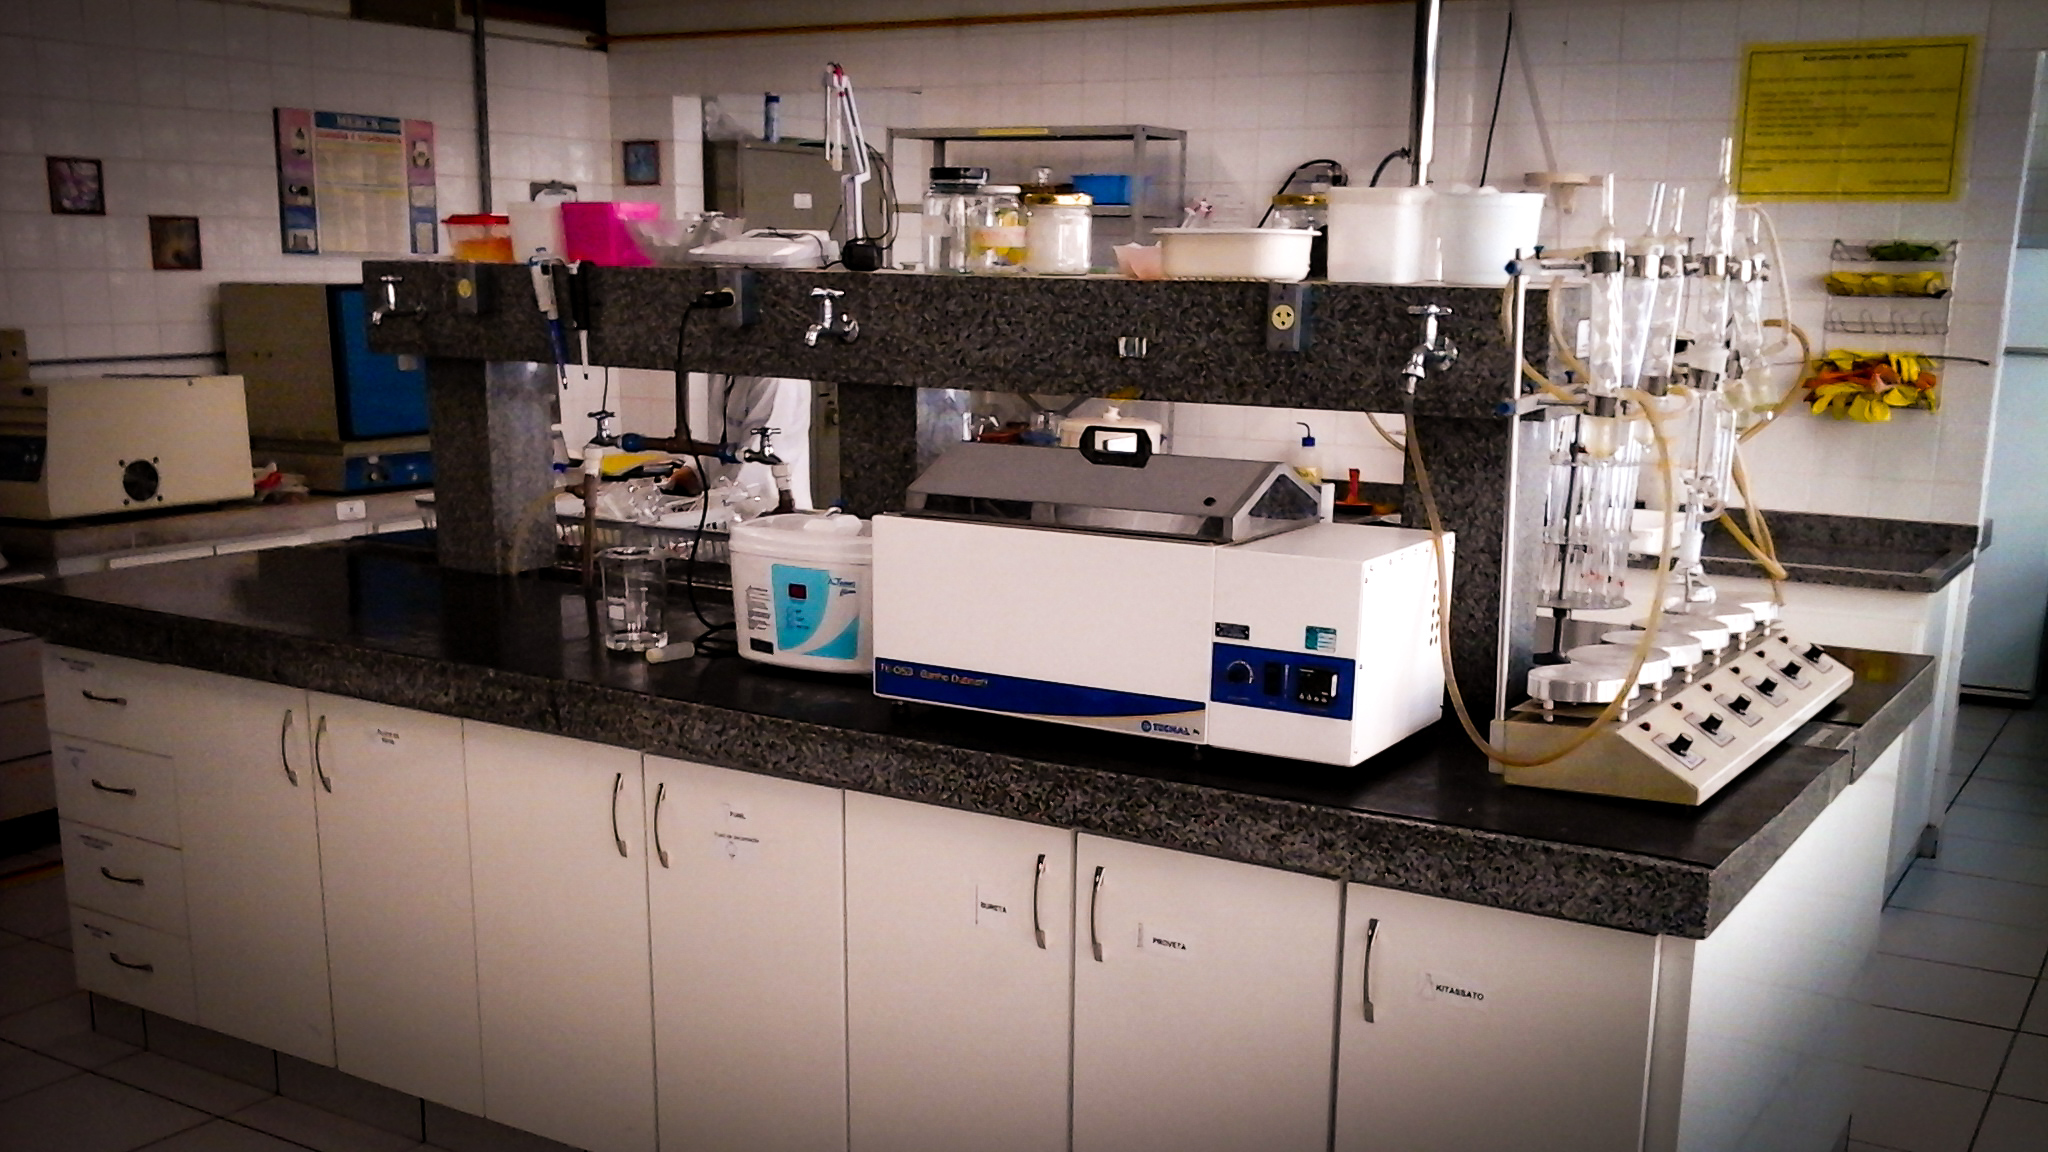
\includegraphics[keepaspectratio]{./imagens/laboratorio.jpg}}

\section{Perigo x Risco}\label{perigo-x-risco}

\subsection{Perigo}\label{perigo}

\begin{itemize}
\item
  Um perigo é o potencial de causar danos, como por exemplo, a
  capacidade de um incêndio de queimar você.

  \begin{itemize}
  \tightlist
  \item
    Por exemplo, vamos considerar o aquecimento de uma cápsula de
    evaporação com um bico de Bunsen.
  \end{itemize}
\end{itemize}

\begin{itemize}
\tightlist
\item
  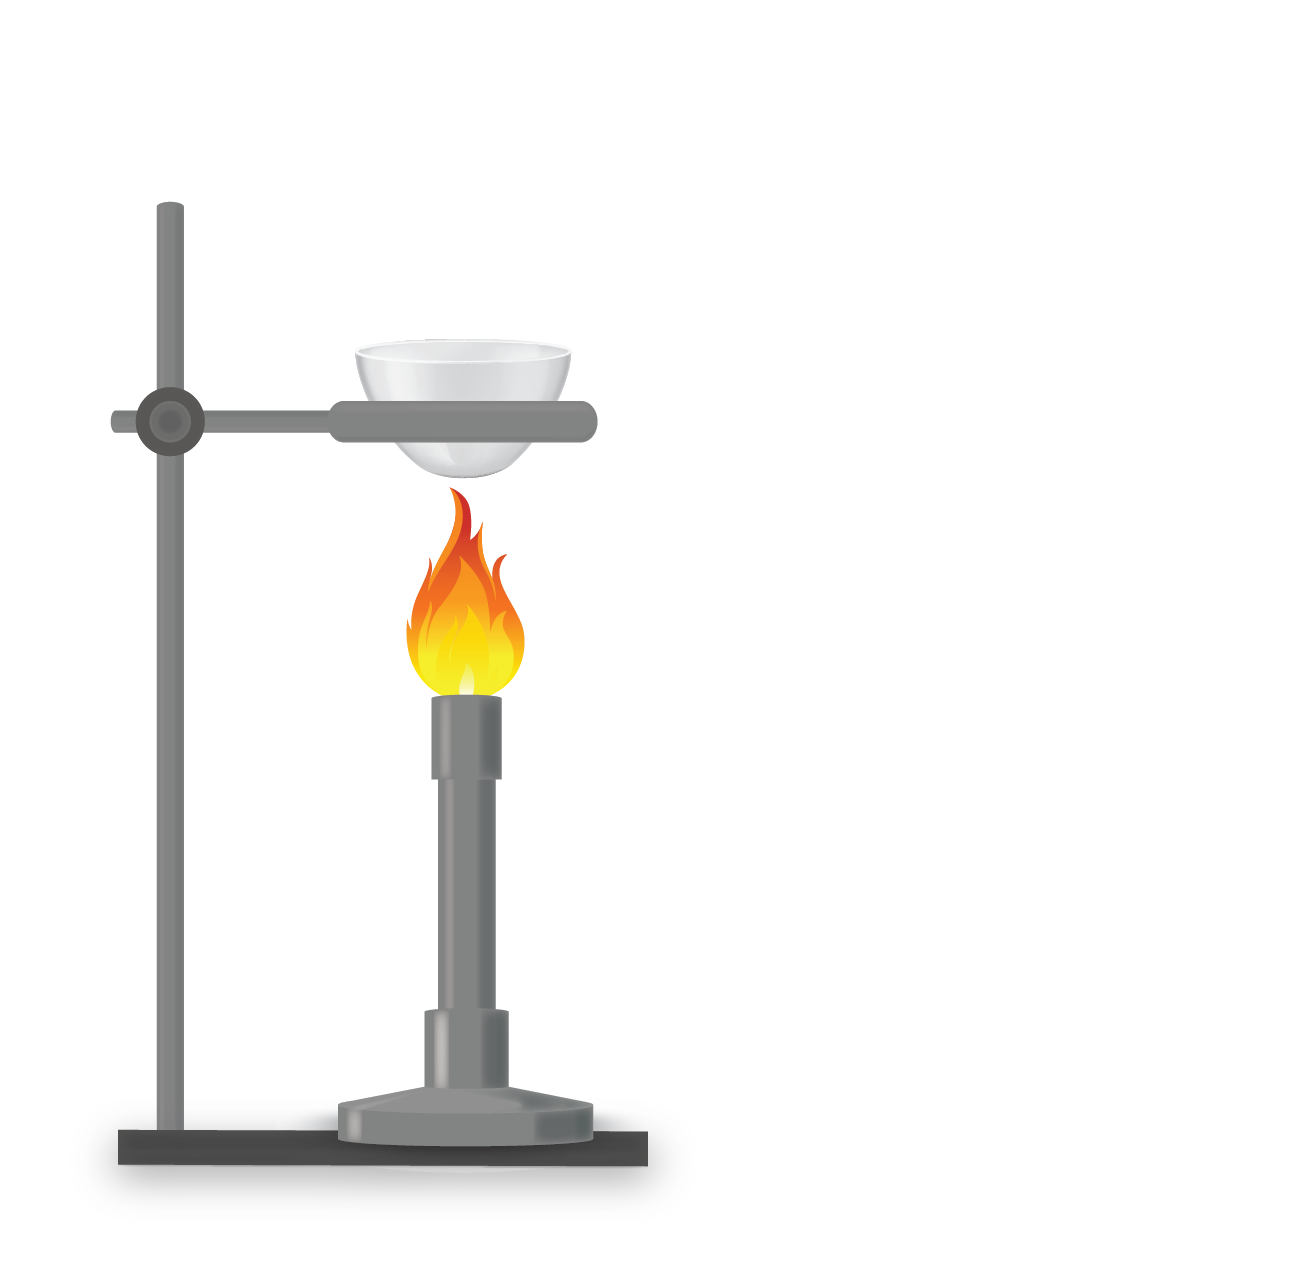
\includegraphics[width=4.16667in,height=\textheight,keepaspectratio]{imagens/image_1.8bbab552.png}
\end{itemize}

\begin{itemize}
\tightlist
\item
  O bico usa uma chama aberta, e o fogo pode queimar você ou inflamar
  materiais combustíveis ou inflamáveis. Isso é um perigo.
\item
  Perigos são propriedades intrínsecas.
\end{itemize}

\subsection{Risco}\label{risco}

\begin{itemize}
\tightlist
\item
  Um risco combina a probabilidade de um evento ocorrer e a sua
  gravidade.
\item
  Se um incêndio vai ou não queimar você é um risco.
\item
  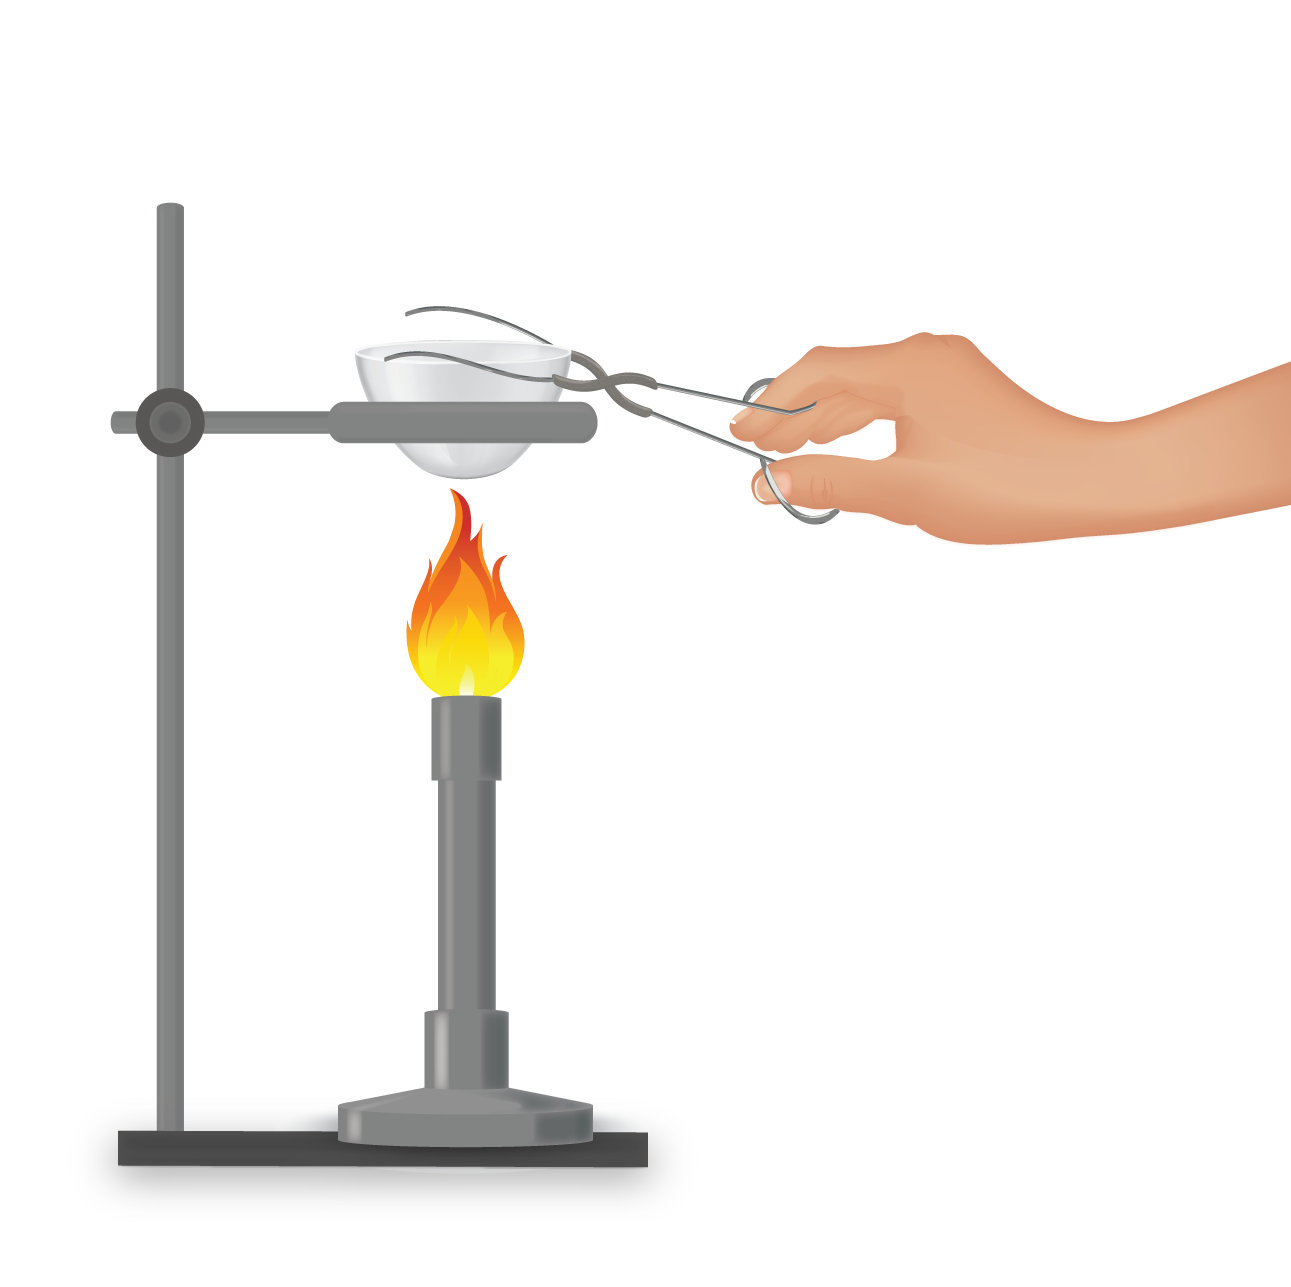
\includegraphics[width=5.20833in,height=\textheight,keepaspectratio]{imagens/image_2.13ea1c26.png}
\end{itemize}

\begin{itemize}
\tightlist
\item
  Ao contrário dos perigos, os riscos podem ser minimizados ou
  eliminados.
\end{itemize}

\subsection{Exemplo Prático}\label{exemplo-pruxe1tico}

Usar roupas folgadas ao trabalhar com uma chama de bico de Bunsen
aumenta o risco de as roupas pegarem fogo.

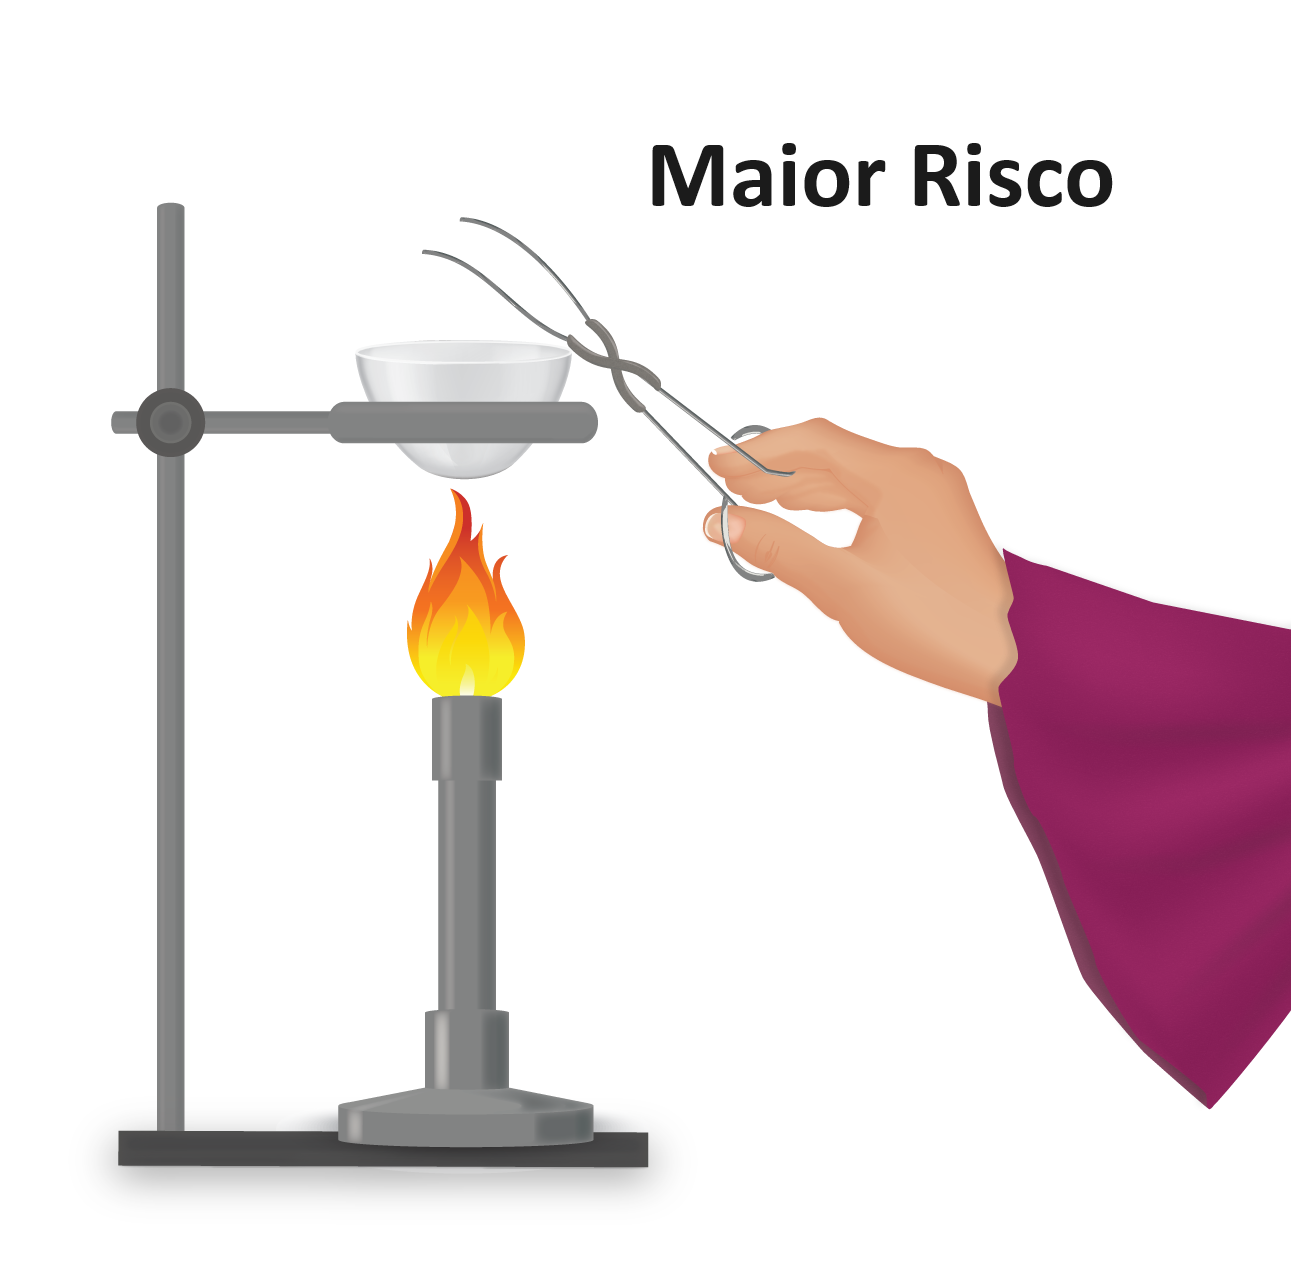
\includegraphics[width=5.20833in,height=\textheight,keepaspectratio]{imagens/image_3.27e26638.png}

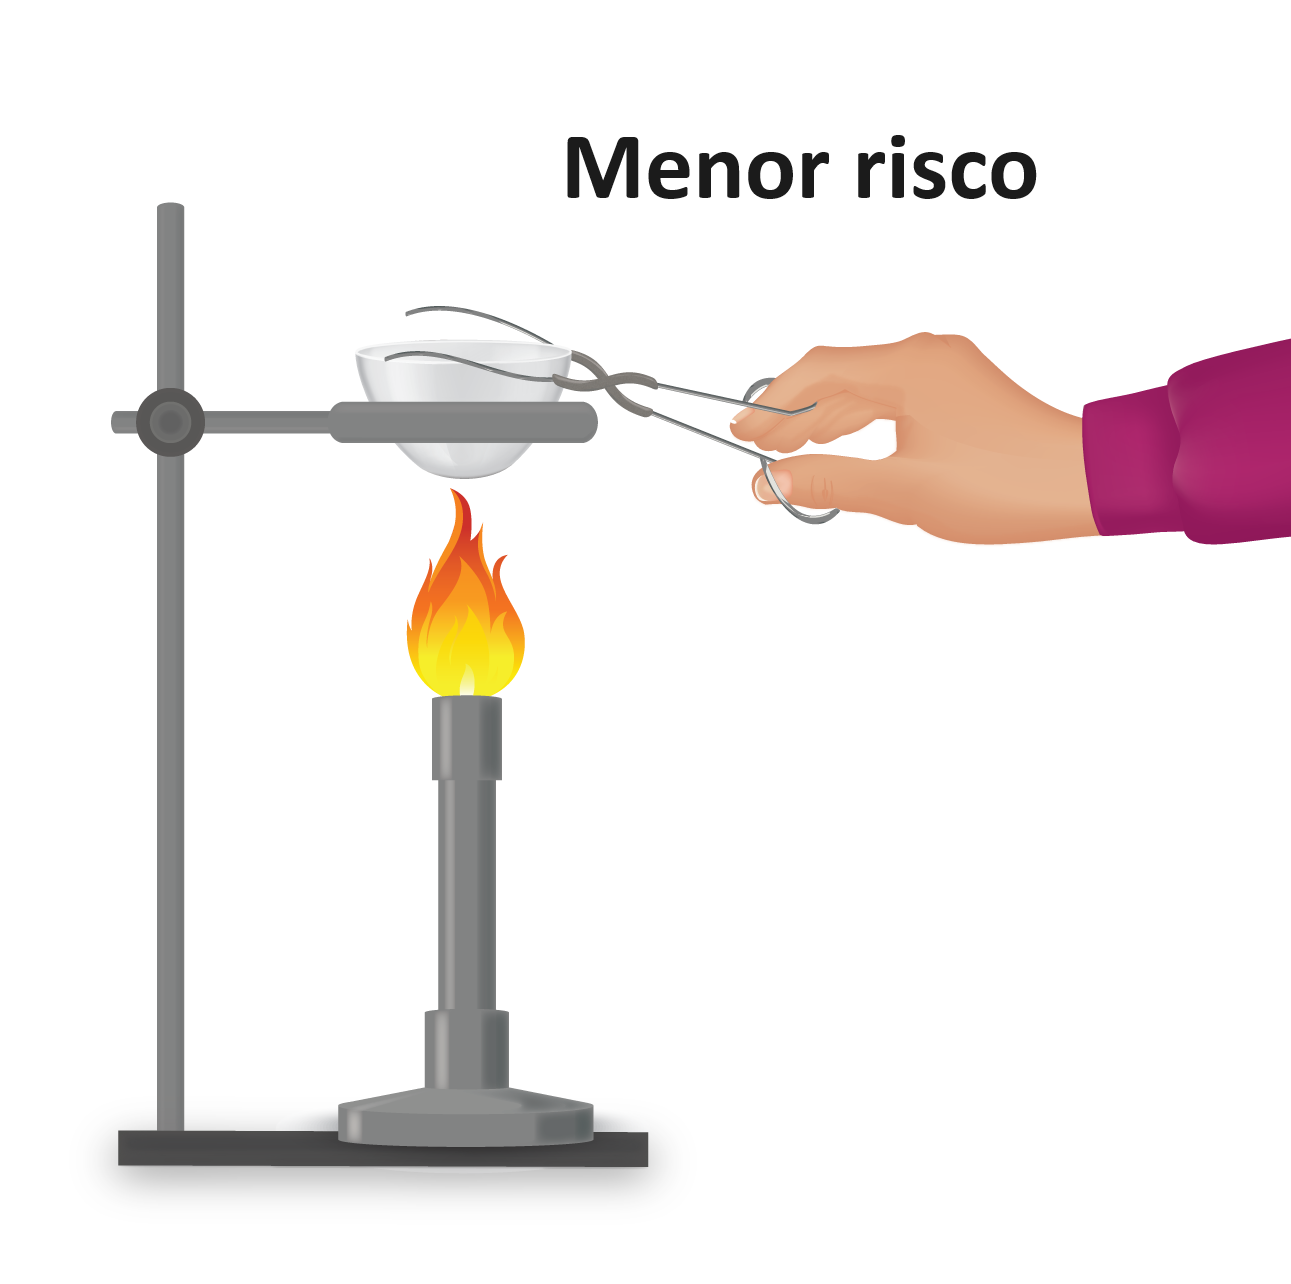
\includegraphics[width=5.20833in,height=\textheight,keepaspectratio]{imagens/image_4.b26a4074.png}

\subsection{Exemplo Prático}\label{exemplo-pruxe1tico-1}

Usar roupas que sejam não-sintéticas e ajustadas minimiza o risco de
ferimentos ou de as roupas pegarem fogo.

\begin{quote}
O perigo ainda está presente, mas o risco foi reduzido.
\end{quote}

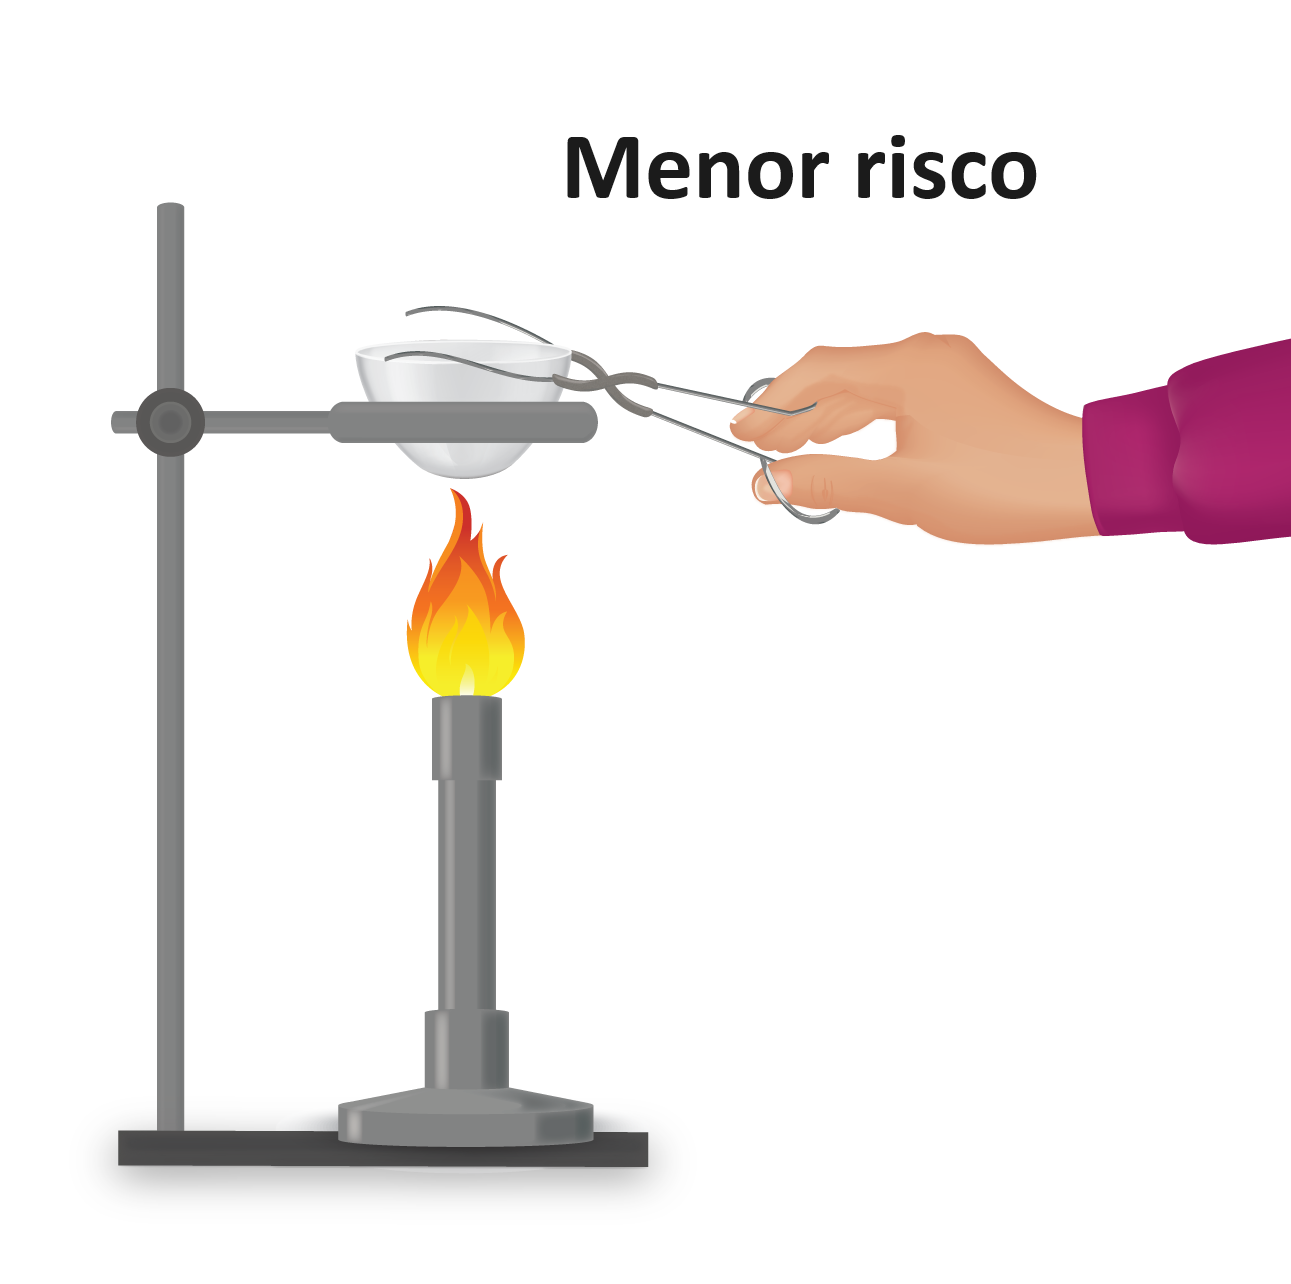
\includegraphics[width=5.20833in,height=\textheight,keepaspectratio]{imagens/image_4.b26a4074.png}

\subsection{Seção de perguntas}\label{seuxe7uxe3o-de-perguntas}

\subsubsection{Dê exemplos de perigos presentes no seu
laboratório}\label{duxea-exemplos-de-perigos-presentes-no-seu-laboratuxf3rio}

\begin{itemize}
\tightlist
\item
  Quais são os níveis de riscos desses perigos?
\item
  Como você pode minimizar esses níveis de riscos?
\item
  Você sabe o que fazer caso os níveis de riscos fiquem sem controle
  (emergência)
\end{itemize}

\section{\texorpdfstring{Os \textbf{agentes químicos} são as principais
\textbf{fontes de perigos} nos laboratórios
químicos}{Os agentes químicos são as principais fontes de perigos nos laboratórios químicos}}\label{os-agentes-quuxedmicos-suxe3o-as-principais-fontes-de-perigos-nos-laboratuxf3rios-quuxedmicos}

\subsection{Para trabalhar em segurança em um laboratório químico, é
necessário:}\label{para-trabalhar-em-seguranuxe7a-em-um-laboratuxf3rio-quuxedmico-uxe9-necessuxe1rio}

\begin{itemize}
\tightlist
\item
  \textbf{R}econhecer os perigos
\end{itemize}

\begin{itemize}
\tightlist
\item
  \textbf{A}valiar os níveis de riscos dos perigos
\end{itemize}

\begin{itemize}
\tightlist
\item
  \textbf{M}inimizar os riscos dos perigos
\end{itemize}

\begin{itemize}
\tightlist
\item
  \textbf{P}reparar-se para as \textbf{emergências} dos \textbf{riscos
  descontrolados}
\end{itemize}

\begin{itemize}
\tightlist
\item
  
\includegraphics[width=6.25in,height=\textheight,keepaspectratio]{imagens/RAMP.png}
\end{itemize}

\begin{itemize}
\tightlist
\item
  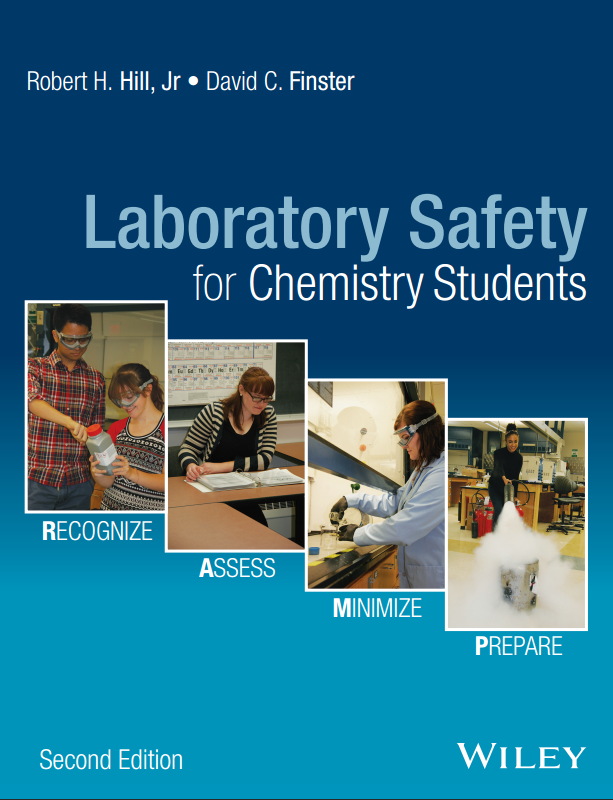
\includegraphics[width=5.20833in,height=\textheight,keepaspectratio]{imagens/hill_e_finster.png}
\end{itemize}

\subsection{O sistema RAMP de segurança
química}\label{o-sistema-ramp-de-seguranuxe7a-quuxedmica}

\begin{itemize}
\tightlist
\item
  
\includegraphics[width=4.16667in,height=\textheight,keepaspectratio]{imagens/RAMP.png}
\item
  Desenvolvido por Robert Hill e David Finster

  \begin{itemize}
  \tightlist
  \item
    Membros dos conselhos de segurança em laboratório da ACS (Sociedade
    Americana de Química)
  \end{itemize}
\item
  É recomendado nas diretrizes da ACS para laboratórios de ensino de
  química dos EUA
\end{itemize}

\begin{itemize}
\item
  \begin{figure}[H]

  {\centering 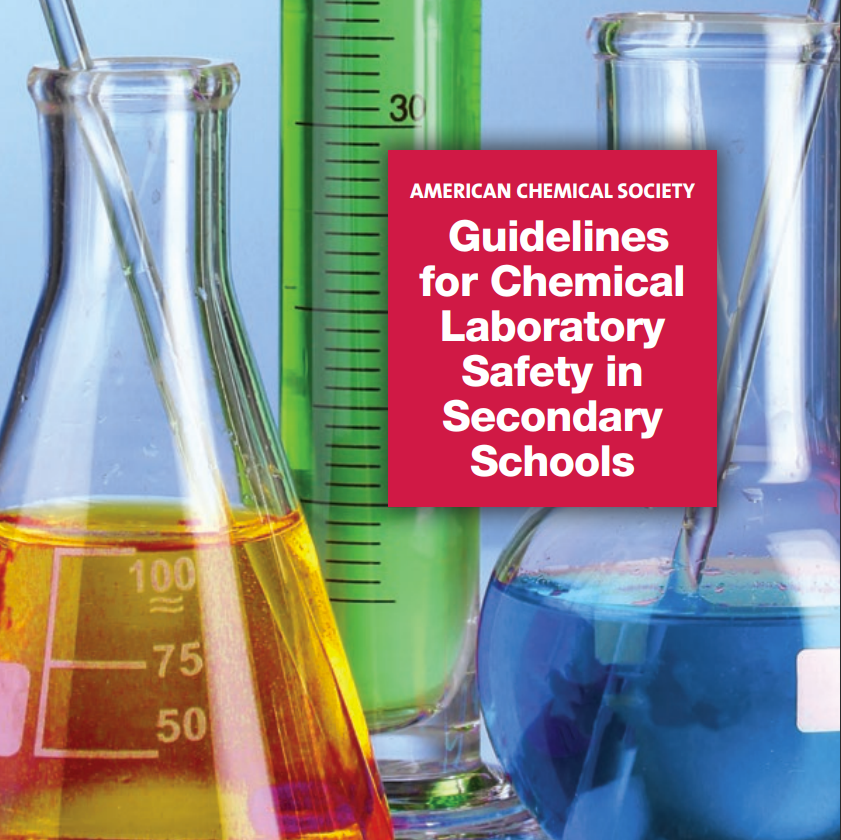
\includegraphics[width=4.375in,height=\textheight,keepaspectratio]{imagens/acs-gss.png}

  }

  \caption{Diretrizes da ACS para os laboratórios de química no ensino
  médio}

  \end{figure}%
\end{itemize}

\begin{itemize}
\item
  \begin{figure}[H]

  {\centering 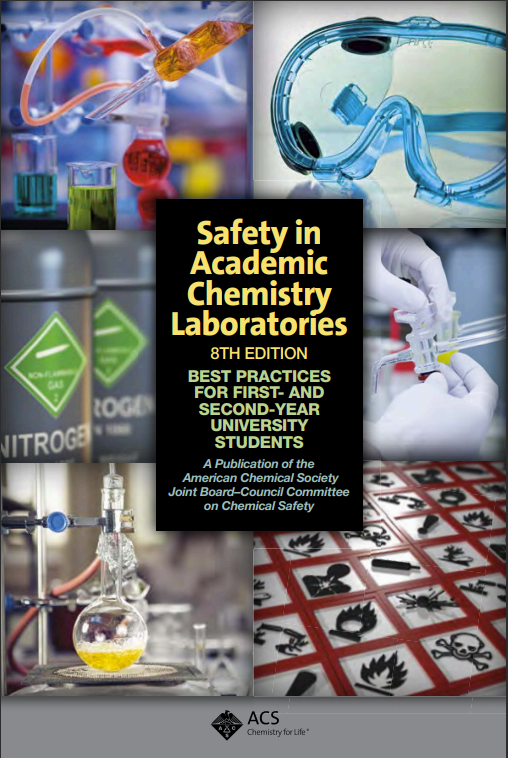
\includegraphics[width=4.375in,height=\textheight,keepaspectratio]{imagens/sacl8.png}

  }

  \caption{Diretrizes da ACS para os laboratórios acadêmicos de química}

  \end{figure}%
\end{itemize}

\subsection{O sistema RAMP no Brasil}\label{o-sistema-ramp-no-brasil}

\begin{itemize}
\tightlist
\item
  A USP ministra a disciplina ``Segurança em Laboratórios de Ensino e
  Pesquisa'' que se baseia no sistema RAMP
\item
  As aulas estão disponíveis online, gratuitamente:
\end{itemize}

\begin{itemize}
\tightlist
\item
  \href{https://edisciplinas.usp.br/course/view.php?id=84617}{Slides}
\item
  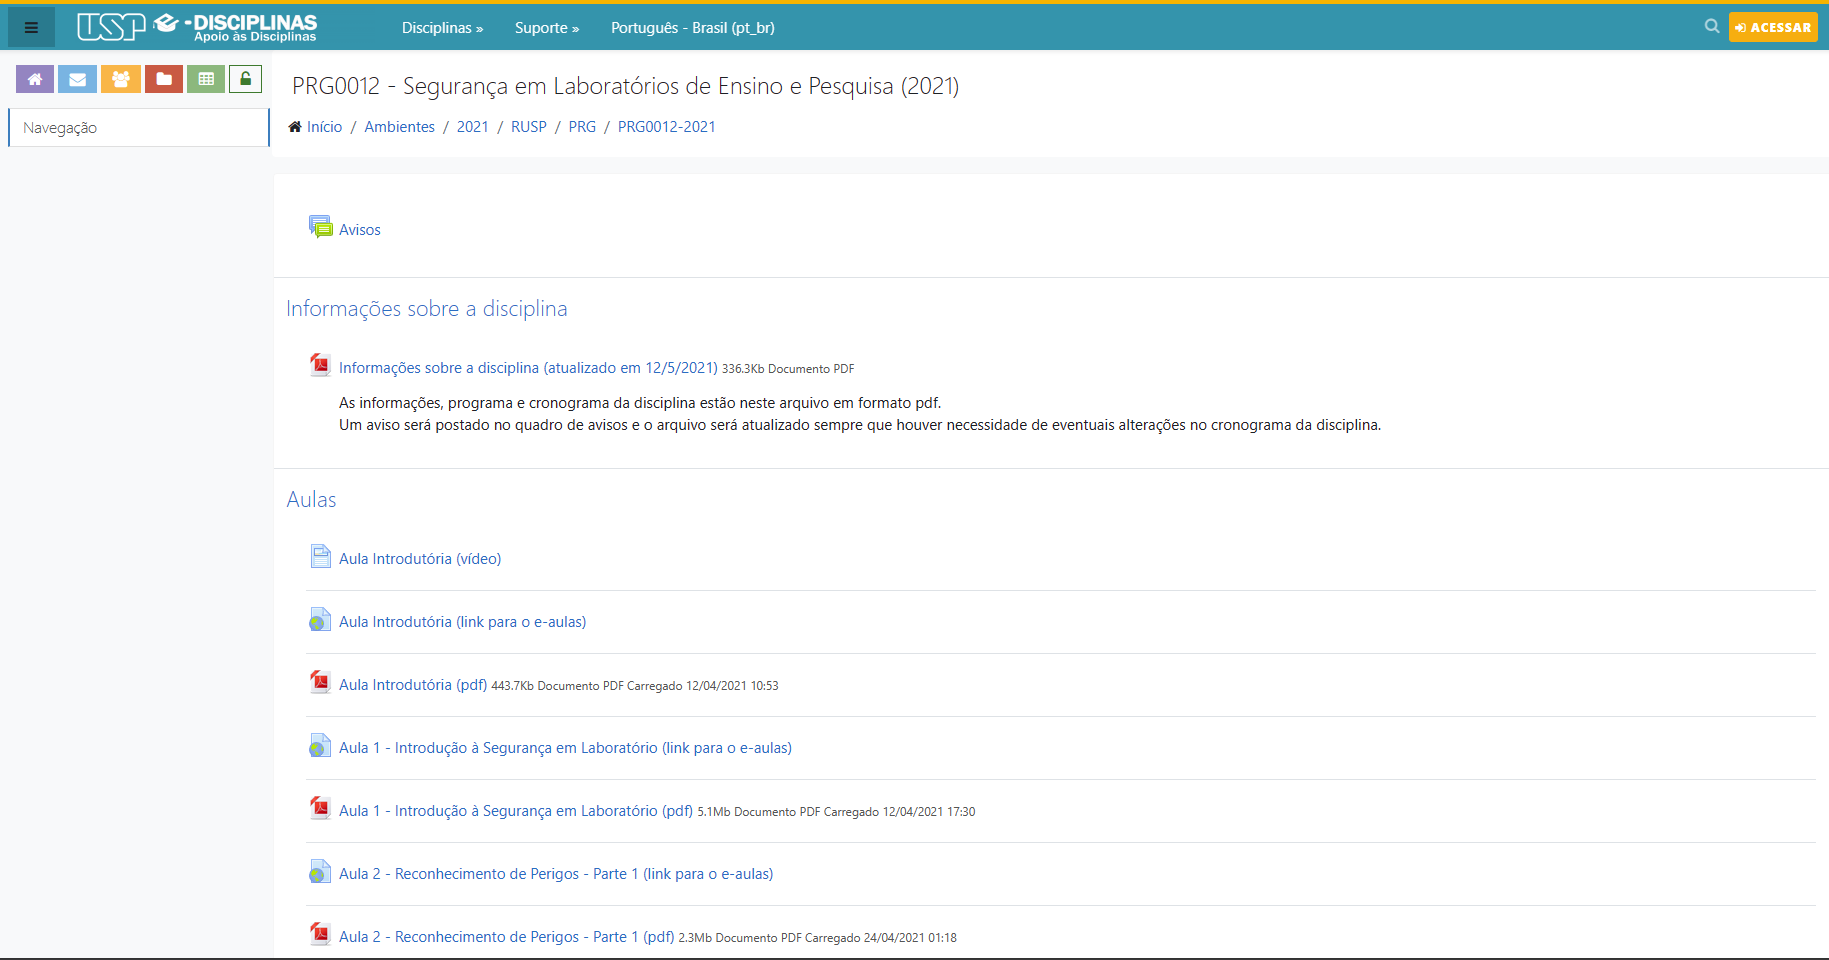
\includegraphics[width=6.25in,height=\textheight,keepaspectratio]{imagens/usp01.png}
\end{itemize}

\begin{itemize}
\tightlist
\item
  \href{https://eaulas.usp.br/portal/course.action?course=24746}{Vídeo
  aulas}
\item
  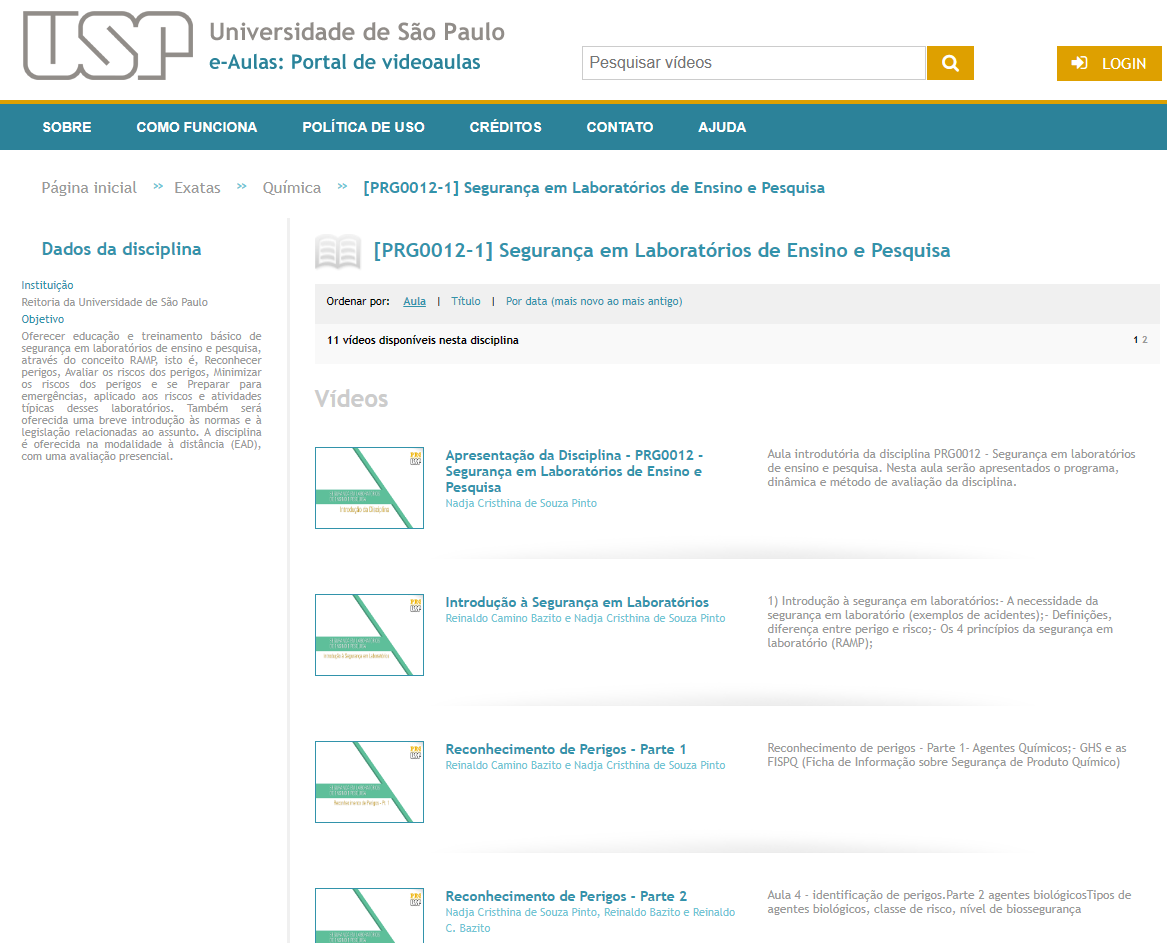
\includegraphics[width=5.20833in,height=\textheight,keepaspectratio]{imagens/usp02.png}
\end{itemize}

\subsection{Seção de perguntas}\label{seuxe7uxe3o-de-perguntas-1}

\subsubsection{Defina os princípios do sistema RAMP de segurança
laboratorial}\label{defina-os-princuxedpios-do-sistema-ramp-de-seguranuxe7a-laboratorial}

\begin{itemize}
\tightlist
\item
  \textbf{R}

  \begin{itemize}
  \tightlist
  \item
    Reconhecer os Perigos
  \end{itemize}
\item
  \textbf{A}

  \begin{itemize}
  \tightlist
  \item
    Avaliar os Riscos
  \end{itemize}
\end{itemize}

\begin{itemize}
\tightlist
\item
  \textbf{M}

  \begin{itemize}
  \tightlist
  \item
    Minimizar os riscos dos perigos
  \end{itemize}
\item
  \textbf{P}

  \begin{itemize}
  \tightlist
  \item
    Preparar-se para as emergências dos riscos não controlados
  \end{itemize}
\end{itemize}

\section{\texorpdfstring{O uso do sistema RAMP contribui para uma
\textbf{cultura de segurança} baseada em \textbf{riscos} e não em
\textbf{regras}}{O uso do sistema RAMP contribui para uma cultura de segurança baseada em riscos e não em regras}}\label{o-uso-do-sistema-ramp-contribui-para-uma-cultura-de-seguranuxe7a-baseada-em-riscos-e-nuxe3o-em-regras}

\subsection{Cultura de Segurança}\label{cultura-de-seguranuxe7a}

\textbf{O que é uma Cultura Compartilhada de Segurança?}

\begin{itemize}
\item
  A segurança tem tanto a ver com crenças e atitudes compartilhadas
  quanto com ameaças físicas.
\item
  Coleção de crenças, valores, percepções e comportamentos sobre riscos
  à saúde e segurança mantidos por uma organização e seus membros como
  uma cultura compartilhada de segurança.
\end{itemize}

\subsection{Cultura de Segurança Baseada em
Regras}\label{cultura-de-seguranuxe7a-baseada-em-regras}

\textbf{Valoriza a aderência às regras}

\begin{itemize}
\item
  As regras de segurança são estabelecidas por autoridades externas ou
  internas, como a Administração de Segurança e Saúde Ocupacional ou um
  membro da faculdade. A instituição depende da fiscalização para
  garantir que seus membros obedeçam às regras de segurança.
\item
  Baixo envolvimento de estudantes e funcionários

  \begin{itemize}
  \tightlist
  \item
    Estudantes e funcionários participam apenas marginalmente na
    definição das regras, portanto, têm pouco compromisso com as regras
    ou compreensão das razões por trás delas.
  \end{itemize}
\end{itemize}

\subsection{Cultura de Segurança Baseada em
Regras}\label{cultura-de-seguranuxe7a-baseada-em-regras-1}

\textbf{Valoriza a aderência às regras}

\begin{itemize}
\item
  Requer grandes investimentos de recursos
\item
  Uma cultura baseada em regras exige treinamento constante e
  requalificação do pessoal. A fiscalização das regras também requer
  grandes quantidades de tempo e atenção.
\item
  Cria percepções negativas sobre precauções de segurança

  \begin{itemize}
  \tightlist
  \item
    As regras parecem arbitrárias e inconvenientes - uma barreira para
    um trabalho eficiente em vez de uma proteção contra incidentes.
    Estudantes e funcionários tendem a desenvolver uma atitude de
    culpabilidade e não se importam ativamente uns com os outros.
  \end{itemize}
\end{itemize}

\subsection{Cultura de Segurança Baseada em
Regras}\label{cultura-de-seguranuxe7a-baseada-em-regras-2}

\textbf{Valoriza a aderência às regras}

\begin{itemize}
\item
  Não é facilmente adaptável a novas situações
\item
  As regras são escritas para perigos conhecidos: uma operação de
  laboratório de rotina, uma operação comum em oficinas, e assim por
  diante. Quando uma nova situação se desenvolve, como um experimento
  inovador, as regras existentes muitas vezes não abrangem a situação,
  parecem excessivamente cautelosas ou especificam ações que são
  potencialmente perigosas.
\end{itemize}

\subsection{Cultura de Segurança Baseada em
Risco}\label{cultura-de-seguranuxe7a-baseada-em-risco}

\textbf{Mantém o foco no risco, não nas regras}

\begin{itemize}
\tightlist
\item
  Embora leis e regulamentos aplicáveis sejam seguidos, as pessoas
  concentram sua atenção em minimizar o risco em vez de memorizar
  regras.
\end{itemize}

\textbf{As avaliações de risco são compartilhadas}

\begin{itemize}
\tightlist
\item
  A tolerância ao risco é definida em conjunto por todos os membros da
  organização, não apenas por um gerente ou regulador. Todos contribuem.
\end{itemize}

\textbf{Requer menos recursos}

\begin{itemize}
\tightlist
\item
  Ensinar conceitos de risco que apoiam as regras de segurança requer
  menos tempo e dinheiro do que a fiscalização constante das regras e a
  requalificação.
\end{itemize}

\subsection{Cultura de Segurança Baseada em
Risco}\label{cultura-de-seguranuxe7a-baseada-em-risco-1}

\textbf{Cria uma atitude positiva em relação à segurança}

\begin{itemize}
\tightlist
\item
  Como as pessoas entendem as razões por trás dos esforços de
  minimização de riscos, estudantes e funcionários passam a se preocupar
  ativamente com a própria segurança e a segurança uns dos outros.
\end{itemize}

\textbf{É adaptável a novas condições}

\begin{itemize}
\tightlist
\item
  Quando os trabalhadores de laboratório podem reconhecer perigos,
  estimar riscos e identificar medidas para minimizar esses riscos, eles
  respondem a novos perigos e situações de maneira previsível, segura e
  mais competente.
\end{itemize}

\subsection{Resumindo}\label{resumindo}

\subsubsection{Cultura baseada em risco}\label{cultura-baseada-em-risco}

\begin{itemize}
\tightlist
\item
  Pesquisadores educados para minimizar o risco
\item
  Cultura lida facilmente com situações novas
\item
  Colaboração favorecida em vez de fiscalização
\item
  Ênfase na redução do risco
\item
  Menos políticas, mais gerais
\end{itemize}

\subsubsection{Cultura baseado em
regras}\label{cultura-baseado-em-regras}

\begin{itemize}
\tightlist
\item
  Pesquisadores treinados em requisitos
\item
  Muitas políticas de segurança
\item
  Ênfase na conformidade com leis e regulamentos
\item
  Muitas inspeções de laboratório
\end{itemize}

\subsection{Relembrando os conceitos}\label{relembrando-os-conceitos}

\begin{itemize}
\item ~
  \subsubsection{Risco x Perigo}\label{risco-x-perigo}
\item ~
  \subsubsection{Sistema de segurança
  RAMP}\label{sistema-de-seguranuxe7a-ramp}
\item ~
  \subsubsection{Cultura de Regras x Cultura de
  Riscos}\label{cultura-de-regras-x-cultura-de-riscos}
\end{itemize}

\section{Perguntas, sugestões,
críticas?}\label{perguntas-sugestuxf5es-cruxedticas}




\end{document}
